To produce predictions for the DCOs that are detectable with LISA, we synthesise a population of DCOs using the population synthesis methods described in Section~\ref{sec:COMPAS_explained}. In order to obtain value for the uncertainty on the expected detection rates, we place this sample of DCOS in many different Monte Carlo sampled instances of the Milky Way, the model for which is described in Section~\ref{sec:galaxy_synthesis}. We evolve the orbit of each DCO in a Milky Way instance up to the LISA mission and calculate the detection rate for that instance using the methods presented in Section~\ref{sec:gw_detection}.

\subsection{Binary population synthesis}\label{sec:COMPAS_explained}

We use the grid of binary population synthesis simulations recently presented in \citet{Broekgaarden+2021} and Broekgaarden et al. (in prep). This grid of simulations is synthesised using the rapid population synthesis code \href{https://compas.science}{COMPAS} \citep{Stevenson+2017, Vigna-Gomez+2018, Stevenson+2019}. COMPAS follows the approach of the pioneering population synthesis code BSE \citep{Hurley+2000,Hurley+2002} and uses fitting formula and rapid algorithms to efficiently predict the final fate of binary systems. The code is open source and documented in the papers listed above, the online documentation\footnote{\url{https://compas.science}} and in the upcoming methods paper (Team COMPAS: J. Riley et al. (in prep)). We summarise the main assumptions and settings relevant for this work in Appendix~\ref{app:pop_synth}.

The result of the simulations is a sample of binaries, which, for each metallicity $Z$, have the parameters
\begin{equation}
    \mathbf{b}_{{Z, i}} = \{m_1, m_2, a_{\rm DCO}, e_{\rm DCO}, t_{\rm evolve}, t_{\rm inspiral}, w\},
\end{equation}
for $i = 1, 2, \dots, N_{\rm binary}$, where $m_1$ and $m_2$ are the primary and secondary masses, $a_{\rm DCO}$ and $e_{\rm DCO}$ are the semi-major axis and eccentricity at the moment of double compact object (DCO) formation, $t_{\rm evolve}$ is the time between the binary's zero-age main sequence and DCO formation, $t_{\rm inspiral}$ is the time between DCO formation (that is immediately after the second supernova in the system) and gravitational wave merger, $w$ is the adaptive importance sampling weight assigned by STROOPWAFEL \cite[][Eq.~7]{Broekgaarden+2019}. We sample from these sets of parameters when creating synthetic galaxies.

\subsection{Galaxy synthesis}\label{sec:galaxy_synthesis}

In order to estimate a detection rate of DCOs with statistical uncertainties, we create a series of random instances of the Milky Way, each populated with a subsample drawn (with replacement) from the synthesised binaries described in Section~\ref{sec:COMPAS_explained}.

Most previous studies that predict a detection rate for LISA place binaries in the Milky Way independently of their age or evolution. We improve upon this as the first study to use an empirically-informed analytical model of the Milky Way that takes into account the galaxy's enrichment history by applying the metallicity-radius-time relation from \citet{Frankel+2018}. The authors developed this relation in order to measure the global efficiency of radial migration in the Milky Way and calibrated it using a sample of red clump stars measured with APOGEE \citep{Majewski+2017}.

In Section~\ref{sec:mw_model}, we outline our model for the Milky Way and in Section~\ref{sec:combining_pop_gal} we explain how we combine our population of synthesised DCOs with this Milky Way model.

\subsubsection{Milky Way model}\label{sec:mw_model}

\begin{figure*}[t]
    \centering
    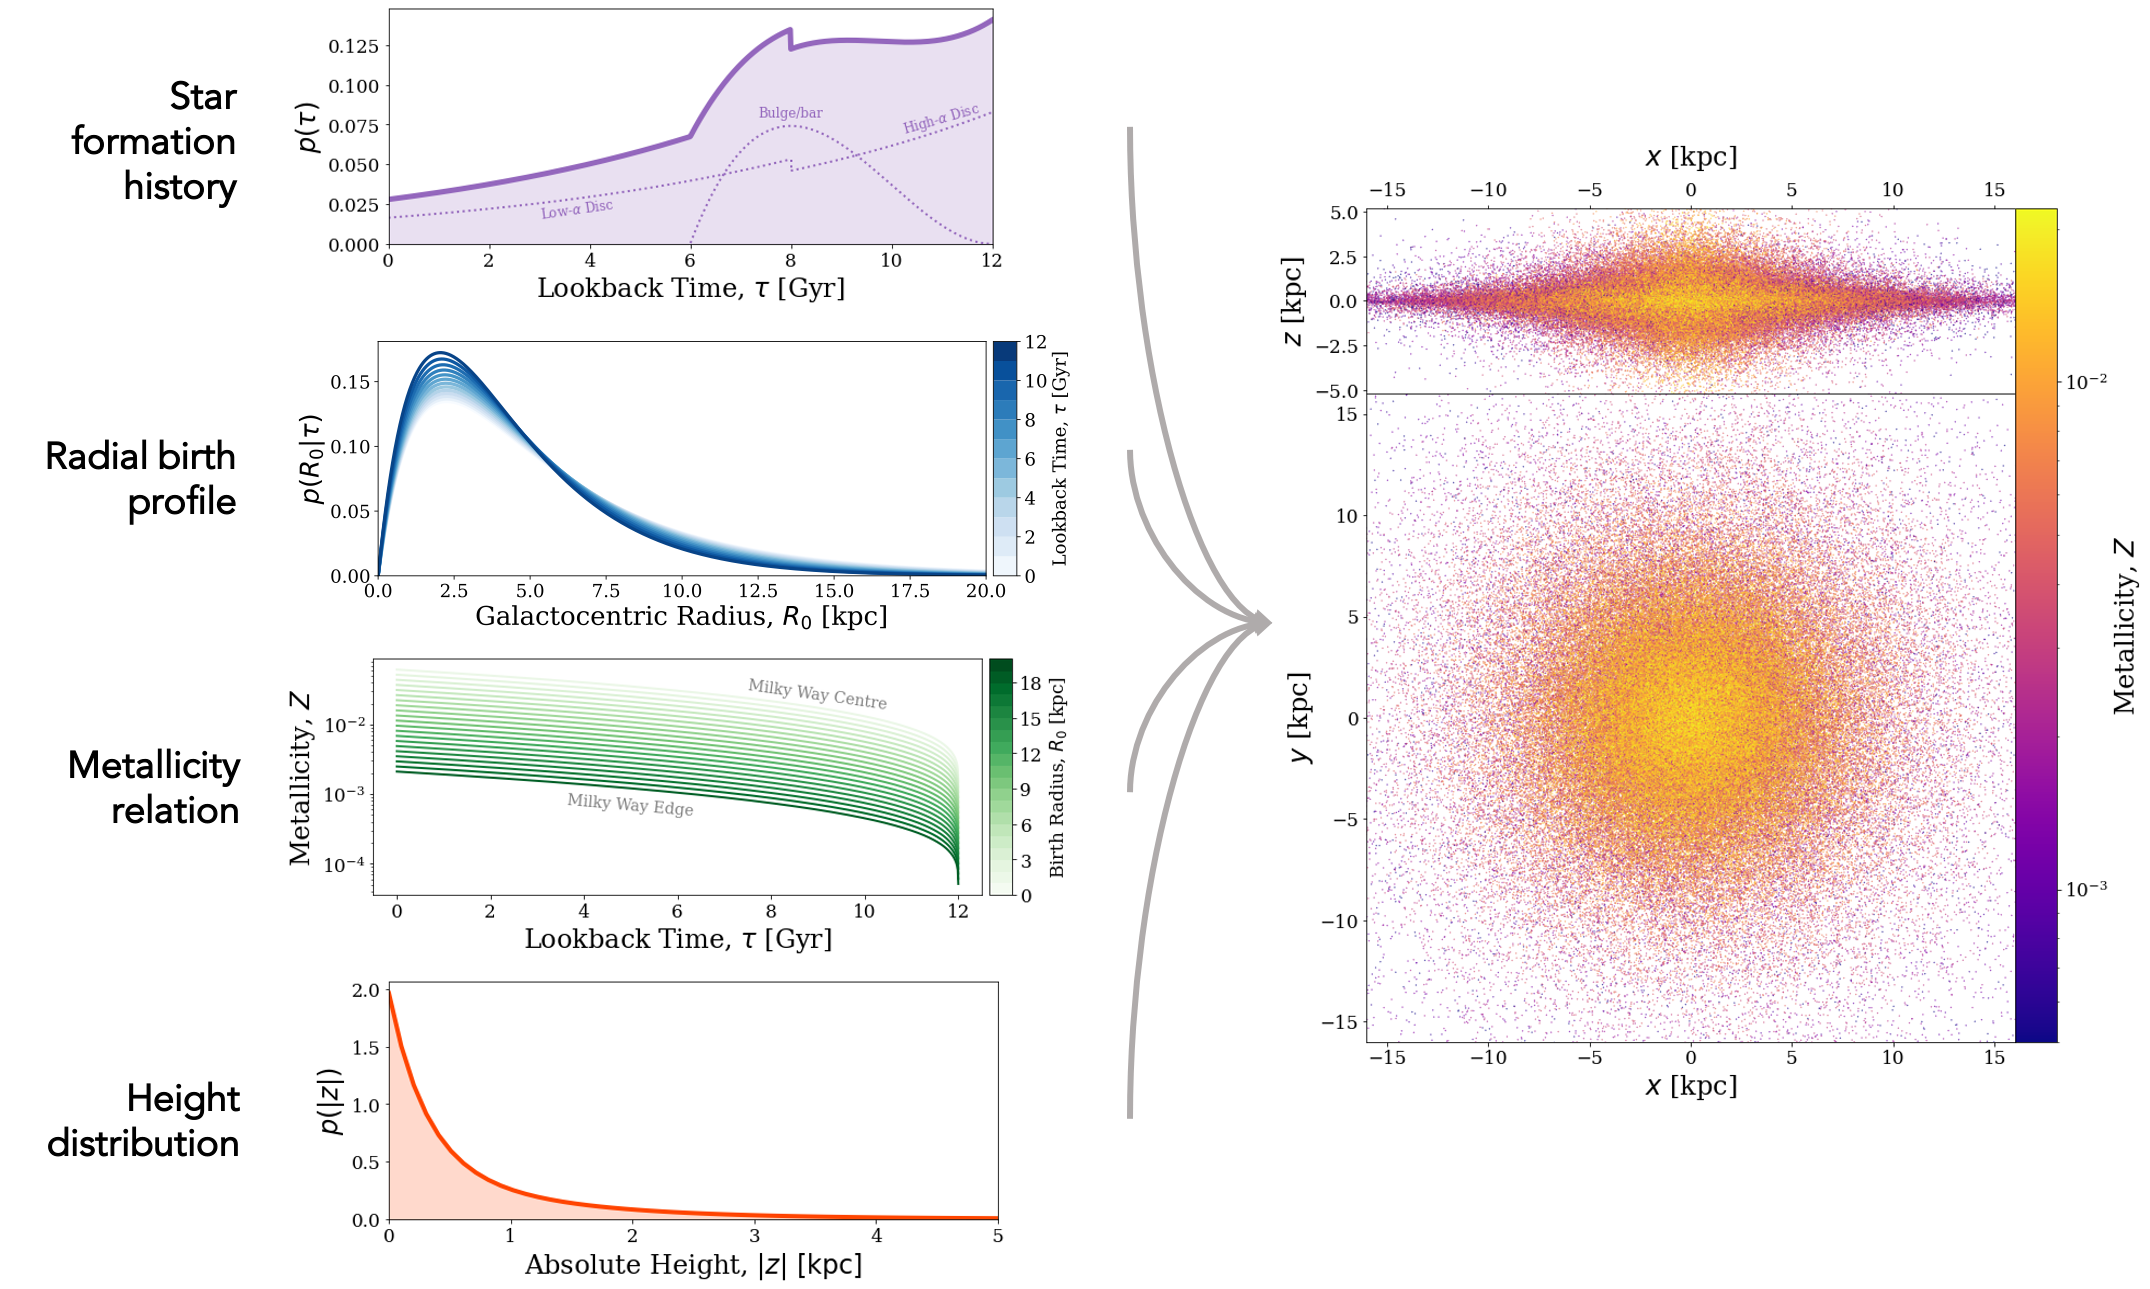
\includegraphics[width=\textwidth]{1_galaxy_diagram.png}
    \caption{A schematic illustrating how we create a mock Milky Way galaxy. The left panel illustrates the different model aspects: star formation history of 3 galactic components (individually shown in the dotted lines), spatial distribution at birth, age-metallicity-radius relation, and vertical distribution.
    On the right, we show an example instance of the Milky Way with $250000$ binaries shown as points colour coded by metallicity. The top panel shows a side-on view and the bottom panel shows a face-on view.}
    \label{fig:galaxy_schematic}
\end{figure*}

Our model for the Milky Way accounts for the low-\achem\footnote{nomenclature used to describe the enhancement of $\alpha$ elements compared to iron in stellar atmospheres}~disc, high-\achem~disc and a central component approximating a bar/bulge. The low- and high-\achem~discs are often also referred to as the thin and thick discs because the stellar vertical distribution is better fit by a double exponential rather than a single one. However, it doesn't allow one to assign a star to either the thin or thick disk purely based on its height above the Galactic plane. Therefore, we use the chemical definition of the two disks with the \achem~nomenclature because there is a clear bimodal distribution in the chemical plane, allowing stars to be easily assigned to each of the disc components based on its chemical abundances. For each of the three components, we use a separate star formation history, radial and vertical distribution, which we combine into a single model, weighting each component by its stellar mass. \citet{Licquia+2015} gives that the stellar mass of the bulge is $0.9 \times 10^{10} \unit{M_{\odot}}$ and the stellar mass of the disc is $5.2 \times 10^{10} \unit{M_\odot}$, which we split equally between the low- and high-\achem~discs \citep[e.g.,][]{Snaith+2014}.

\textit{Star formation history:} 
We use an exponentially declining star formation history \citep{Frankel+2018} (a priori inspired by average the cosmic star formation history) for the combined low- and high-\achem~discs, where the two discs transition at about 8 Gyr ago, and re-normalize the produced mass to be equal in each of the two components.
\begin{equation}\label{eq:thin_disc_tau}
    p(\tau) \propto \exp \qty(-\frac{(\tau_m - \tau)}{\tau_{\rm SFR}}),
\end{equation}
where $\tau$ is the lookback time (the amount of time elapsed between the binary's zero-age main sequence and today), $\tau_m = 12 \unit{Gyr}$ is the assumed age of the Milky Way and $\tau_{\rm SFR} = 6.8 \unit{Gyr}$ is the star formation timescale. 

The star formation history of the Milky Way bulge (which we assume here to be dominated by the central bar) has many uncertainties due to (1) sizeable age measurement uncertainties at large ages in observational studies, (2) complex selection processes affecting the observed age distributions, and (3) formation mechanisms still under debate. But the central bar was shown to contain stars with an age range of 6-12 Gyr \citep[e.g.,][]{Bovy+2019}, where the younger tail of ages might come from the growth of the Galactic bar. To model the bar's age distribution more realistically than in previous studies (assuming an old bulge coming from a single starburst), we choose to adopt a star formation history using a $\beta(2,3)$ distribution, shifted and scaled such that stars are only formed in the range $[6, 12] \unit{Gyr}$. We show these distributions in the first panel in the left half of Fig.~\ref{fig:galaxy_schematic}.

\textit{Radial distribution:} For each of the three components we employ the same single exponential distribution (but with different scale lengths)
\begin{equation}\label{eq:galaxy_R}
    p(R) = \exp(-\frac{R}{R_d}) \frac{R}{R_d^2},
\end{equation}
where $R$ is the Galactocentric radius and $R_d$ is the scale length of the component. For the low-\achem~disc, we set $R_d = R_{\rm exp}(\tau)$, where $R_{\rm exp}(\tau)$ is the scale length presented in \citet[][Eq.~5]{Frankel+2018}
\begin{equation}
    R_{\rm exp}(\tau) = 4 \unit{kpc} \qty(1 - \alpha_{R_{\rm exp}} \qty(\frac{\tau}{8 \unit{Gyr}})),
\end{equation}
where $\alpha_{R_{\rm exp}} = 0.3$ is the inside-out growth parameter\footnote{In $R_{\rm exp}(\tau)$, we use 4 kpc instead of 3 kpc for the 0 Gyr exponential scale-length of the disc as NF finds that it provides a better fit to the original data}. This scale length accounts for the inside-out growth of the low-\achem~disc and hence is age dependent. We assume $R_d = (1 / 0.43) \unit{kpc}$ for the high-\achem~disc \citep[][Table~1]{Bovy+2016} and $R_d = 1.5 \unit{kpc}$ for the bar component \citep{Bovy+2019}. We show the combination of these distributions in the second panel in the left half of Fig.~\ref{fig:galaxy_schematic}.

\textit{Vertical distribution}: Similar to the radial distribution, we use the same single exponential distribution (but with different scale heights) for each component
\begin{equation}\label{eq:galaxy_z}
    p(\abs{z}) = \frac{1}{z_d} \exp\qty(-\frac{z}{z_d}),
\end{equation}
where $z$ is the height above the Galactic plane and $z_d$ is the scale height. We set $z_d = 0.3 \unit{kpc}$ for the low-\achem~disc \citep{McMillan+2011} and $z_d = 0.95 \unit{kpc}$ for the high-\achem~disc \citep{Bovy+2016}. 
For the bar, we set $z_d = 0.2 \unit{kpc}$ \citep{Wegg+15}. We show the combination of these distributions in the last panel in the left half of Fig.~\ref{fig:galaxy_schematic}.

\textit{Metallicity-radius-time relation:} To account for the chemical enrichment of star forming gas as the Milky Way evolves, we adopt the relation given by \citep[][Eq. 7]{Frankel+2018}
\begin{equation}\label{eq:galaxy_FeH}
    \begin{split}
        [{\rm Fe} / {\rm H}] (R, \tau) &= F_m + \nabla [{\rm Fe} / {\rm H}] R \\
        &- \qty(F_m + \nabla [{\rm Fe} / {\rm H}] R^{\rm now}_{[{\rm Fe} / {\rm H}] = 0} ) f(\tau),
    \end{split}
\end{equation}
where
\begin{equation}
    f(\tau) = \qty(1 - \frac{\tau}{\tau_m})^{\gamma_{[{\rm Fe} / {\rm H}]}},
\end{equation}
$F_m = -1 \unit{dex}$ is the metallicity of the gas at the center of the disc at $\tau = \tau_m$, $\nabla [{\rm Fe} / {\rm H}] = -0.075 \unit{kpc^{-1}}$ is the metallicity gradient, $R^{\rm now}_{[{\rm Fe} / {\rm H}] = 0} = 8.7 \unit{kpc}$ is the radius at which the present day metallicity is solar and $\gamma_{[{\rm Fe} / {\rm H}]} = 0.3$ set the time dependence of the chemical enrichment. We can convert this to the representation of metallicity that we use in this paper by applying \citep[e.g][]{Bertelli+1994}
\begin{equation}\label{eq:galaxy_FeH_to_Z}
    \log_{10} (Z) = 0.977 [{\rm Fe} / {\rm H}] + \log_{10}(Z_\odot).
\end{equation}

Although \citet{Frankel+2018} only fit this model for the low-\achem~disc, we also use this metallicity-radius-time relation for the high-$\alpha$ disc and the bar, but focusing on the chemical tracks more representative to the inner disc and large ages. \citet{Sharma+2020} showed that using a simple continuous model for both the low- and high-\achem~discs, the Milky Way abundance distributions could be well reproduced. Empirically, the chemical tracks in the [$\alpha$/Fe]-[Fe/H] plane of the stars in the bulge/bar follow the same track as those of the old stars in the Solar neighbourhood \citep[][Fig.~7,]{Bovy+2019}, which motivates our modelling choice to use the same metallicity-radius-time relation.

Fig.~\ref{fig:galaxy_schematic} shows the distributions and relations outlined in this section and also displays an example random galaxy drawn using this model.

\subsubsection{Combining population and galaxy synthesis}\label{sec:combining_pop_gal}

For each Milky Way instance, we randomly sample the following set of parameters
\begin{equation}
    \mathbf{g}_{{i}} = \{\tau, R, Z, z, \theta\}
\end{equation}
for $i = 1, 2, \dots, N_{\rm MW}$, where we set $N_{\rm MW} = 2 \times 10^{5}$, $\tau, R, Z$ and $z$ are defined and sampled using the distribution functions specified in Section~\ref{sec:mw_model}, $\theta$ is the polar angle sampled uniformly on $[0, 2\pi)$ and $Z$ is the metallicity. Figure~\ref{fig:galaxy_schematic} shows an example of a random Milky Way instance created with these distributions. This shows how these distributions translate to positions in the Milky and illustrates the gradient in metallicity over radius.

We match each set of galaxy parameters $\mathbf{g}_{{i}}$, to a random set of binary parameters $\mathbf{b}_{{Z, i}}$, by drawing a set of binary parameters from the closest metallicity bin to the metallicity in $\mathbf{g}_{{i}}$.

Each binary is likely to move from its birth orbit. Although all stars in the Galactic disc experience radial migration \citep{Sellwood+2002, Frankel+2018}, double compact objects generally experience stronger dynamical evolution as a result of the effects of both Blaauw kicks \citep{Blaauw+1961} and natal kicks \citep[e.g.][]{Hobbs+2005}.

The magnitude of the systemic kicks are typically small compared to the initial circular velocity of a binary at each Galactocentric radius. Therefore, we expect that kicks will not significantly alter the overall distribution of their positions. Given this, and for the sake of computational efficiency, we do not account for the displacement due to systemic kicks in our analysis.

\subsection{Gravitational wave detection}\label{sec:gw_detection}
We use the Python package \href{https://legwork.readthedocs.io/en/latest/}{LEGWORK} to evolve binaries and calculate their LISA detectability. For a full derivation of the equations given below please see the LEGWORK release paper, Wagg et al. 2021b (in prep), or the \href{https://legwork.readthedocs.io/en/latest/notebooks/Derivations.html}{documentation}.

\subsubsection{Inspiral evolution}

Each binary loses orbital energy to gravitational waves throughout its lifetime. This causes the binary to shrink and circularise over time. In order to assess the detectability of a binary, we need to know its eccentricity and frequency at the time of the LISA mission. For each binary in our simulated Milky Way, we know that the time from DCO formation to today is $\tau - t_{\rm evolve}$ and that the initial eccentricity and semi-major axis are $e_{\rm DCO}$ and $a_{\rm DCO}$. We find the eccentricity of the binary at the start of the LISA mission, $e_{\rm LISA}$, by numerically integrating its time derivative \citep[][Eq. 5.13]{Peters+1964} given the initial conditions. This can be converted to the semi-major axis at the start of LISA, $a_{\rm LISA} $\citep[][Eq. 5.11]{Peters+1964}, which in turn gives the orbital frequency, $f_{\rm orb, LISA}$, by Kepler's third law.

\subsubsection{Binary detectability}

We define a binary as detectable if its gravitational wave signal has a signal-to-noise ratio of greater than 7 \citep[e.g.][]{Breivik+2020, Korol+2020}. The sky-, polarisation- and orientation-averaged signal-to-noise ratio, $\rho$, of an inspiraling binary can be calculated with the following \citep[e.g.][]{Finn+2000}
\begin{equation}\label{eq:snr}
    \rho^2 = \sum_{n=1}^{\infty} \int_{f_{n, i}}^{f_{n, f}} \frac{h_{c, n}^{2}}{f_{n}^{2} S_{\rm n}\left(f_{n}\right)} \dd{f_n},
\end{equation}
where $n$ is a harmonic of the gravitational wave signal, $f_n = n \cdot f_{\rm orb}$ is the frequency of the $n^{\rm th}$ harmonic of the gravitational wave signal, $f_{\rm orb}$ is the orbital frequency, $S_{\rm n}(f_n)$ is the LISA sensitivity curve at frequency $f_n$ \citep[e.g.][]{Robson+2019} and $h_{c,n}$ is the characteristic strain of the $n^{\rm th}$ harmonic, given by \citep[e.g.][]{Barack+2004}
\begin{equation}\label{eq:charstrain}
    h^2_{c,n} = \frac{2^{5/3}}{3 \pi^{4/3}} \frac{(G \mathcal{M}_c)^{5/3}}{c^3 D_L^2} \frac{1}{f_{\rm orb}^{1/3}} \frac{g(n,e)}{n F(e)},
\end{equation}
where $D_L$ is the luminosity distance to the source, $f_{\rm orb}$ is the orbital frequency, $g(n, e)$ and $F(e)$ are given in \citet{Peters+1963} and $\mathcal{M}_c$ is the chirp mass, defined as
\begin{equation}\label{eq:chirp_mass}
    \mathcal{M}_c = \frac{(m_1 m_2)^{3/5}}{(m_1 + m_2)^{1/5}}.
\end{equation}

We use LEGWORK to calculate the signal-to-noise ratio for each binary and the package ensures that enough harmonics are computed for each binary such that the error on the gravitational wave luminosity remains below 1\%.

\subsubsection{Detection rate calculation}
For each physics variation model and DCO type, we compute the total number of merging DCOs in the Milky Way today, $N_{\rm MW}$, based on the COMPAS simulation. This takes into account the true mass and IMF of the Milky Way since our simulations may each have a slightly different galaxy mass and only ever sample from massive stars rather than the full IMF. For more details see Appendix~\ref{app:rate_normalisation}.

We determine the fraction of binaries that are detectable in each Milky Way instance by summing the adaptive importance sampling weights of the binaries that have an SNR greater than 7 and dividing by the total weights in the simulation. We multiply this fraction by the total number in the Milky Way to find a detection rate.
\begin{equation}
    N_{\rm detect} = \frac{\sum_{i = 0}^{N_{\rm detect}} w_i}{\sum_{i = 0}^{N_{\rm DCO}} w_i} \cdot N_{\rm MW}
\end{equation}
We calculate the detection rate by Monte Carlo sampling 2500 Milky Way instances (each containing 200,000 DCOs) for each DCO type and every physics variation in order to obtain values for the uncertainty on the expected detection rate.